\documentclass[12pt, twoside]{article}
\usepackage[francais]{babel}
\usepackage[T1]{fontenc}
\usepackage[latin1]{inputenc}
\usepackage[left=6mm, right=6mm, top=6mm, bottom=6mm]{geometry}
\usepackage{float}
\usepackage{graphicx}
\usepackage{array}
\usepackage{multirow}
\usepackage{amsmath,amssymb,mathrsfs}
\usepackage{soul}
\usepackage{textcomp}
\usepackage{eurosym}
 \usepackage{variations}
\usepackage{tabvar}

\begin{document}


\section*{\center{Exercices sur les fonctions}}
 

 
\begin{tabular}{cc}
\begin{minipage}{8cm}
\textbf{Exercice 1}

\enskip

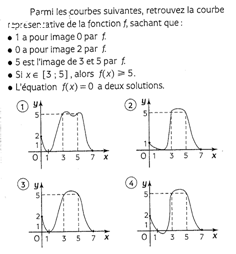
\includegraphics[width=6cm]{images/ex1.png}
\end{minipage} 
&
\begin{minipage}{8cm}
\textbf{Exercice 2}

\enskip

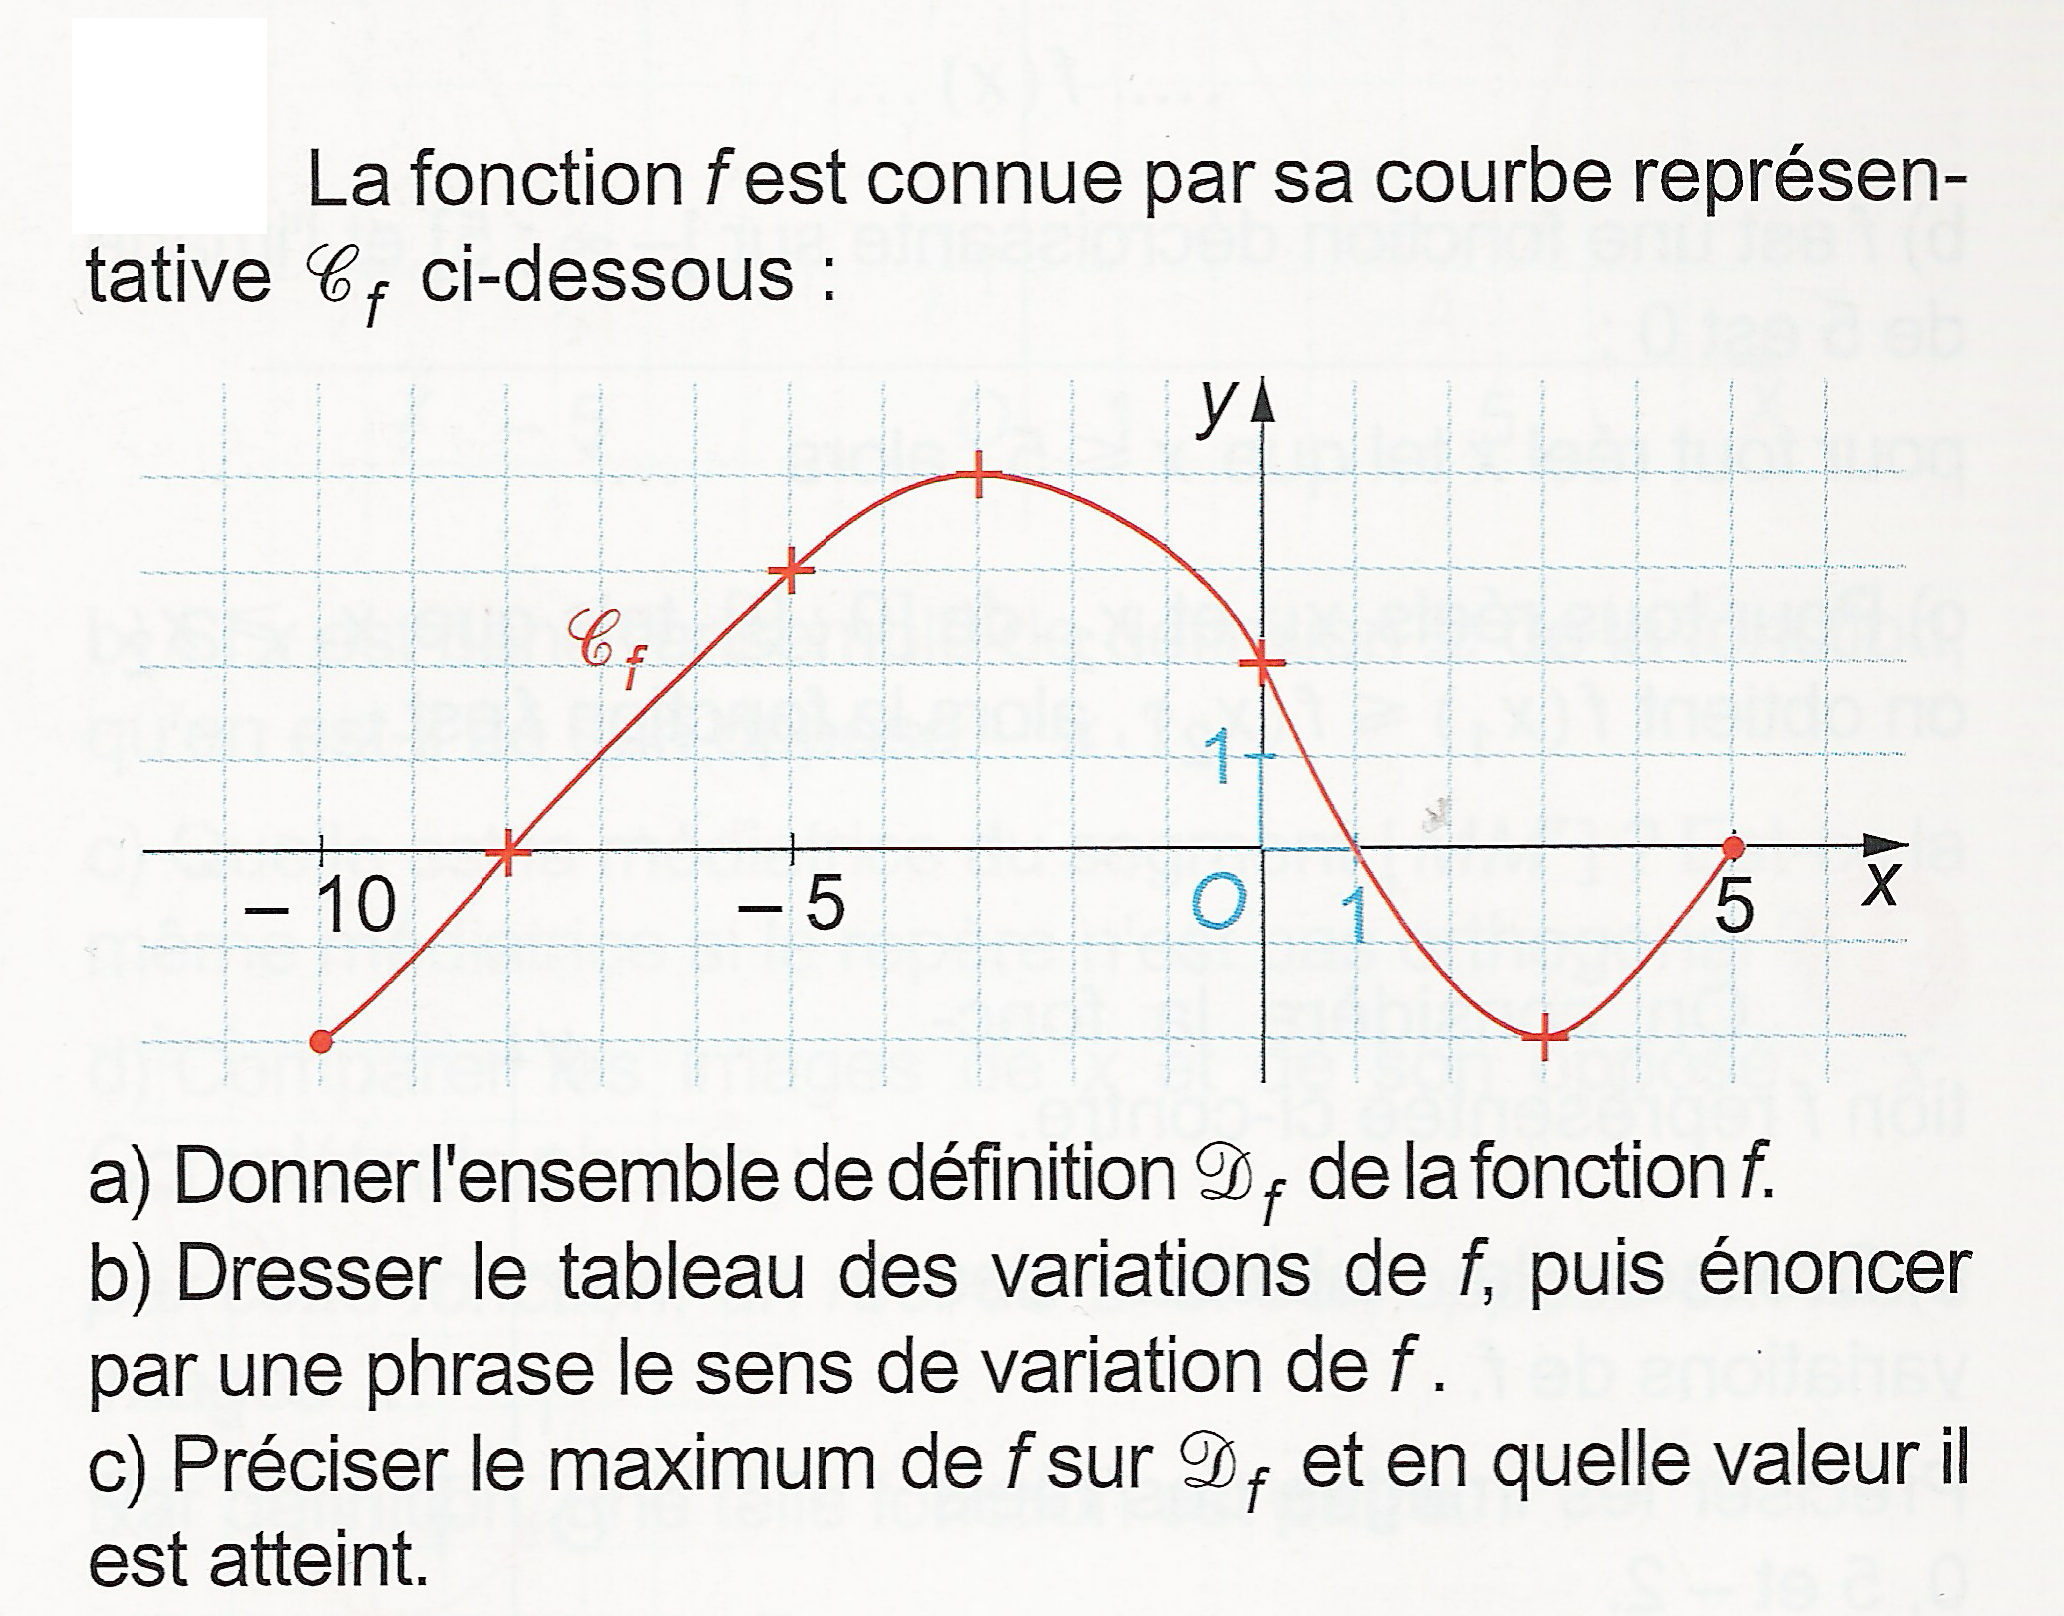
\includegraphics[width=7cm]{images/ex2.png}
\end{minipage}
\end{tabular}

\bigskip
 
\begin{tabular}{cc}
\begin{minipage}{8cm}
\textbf{Exercice 3}

\enskip

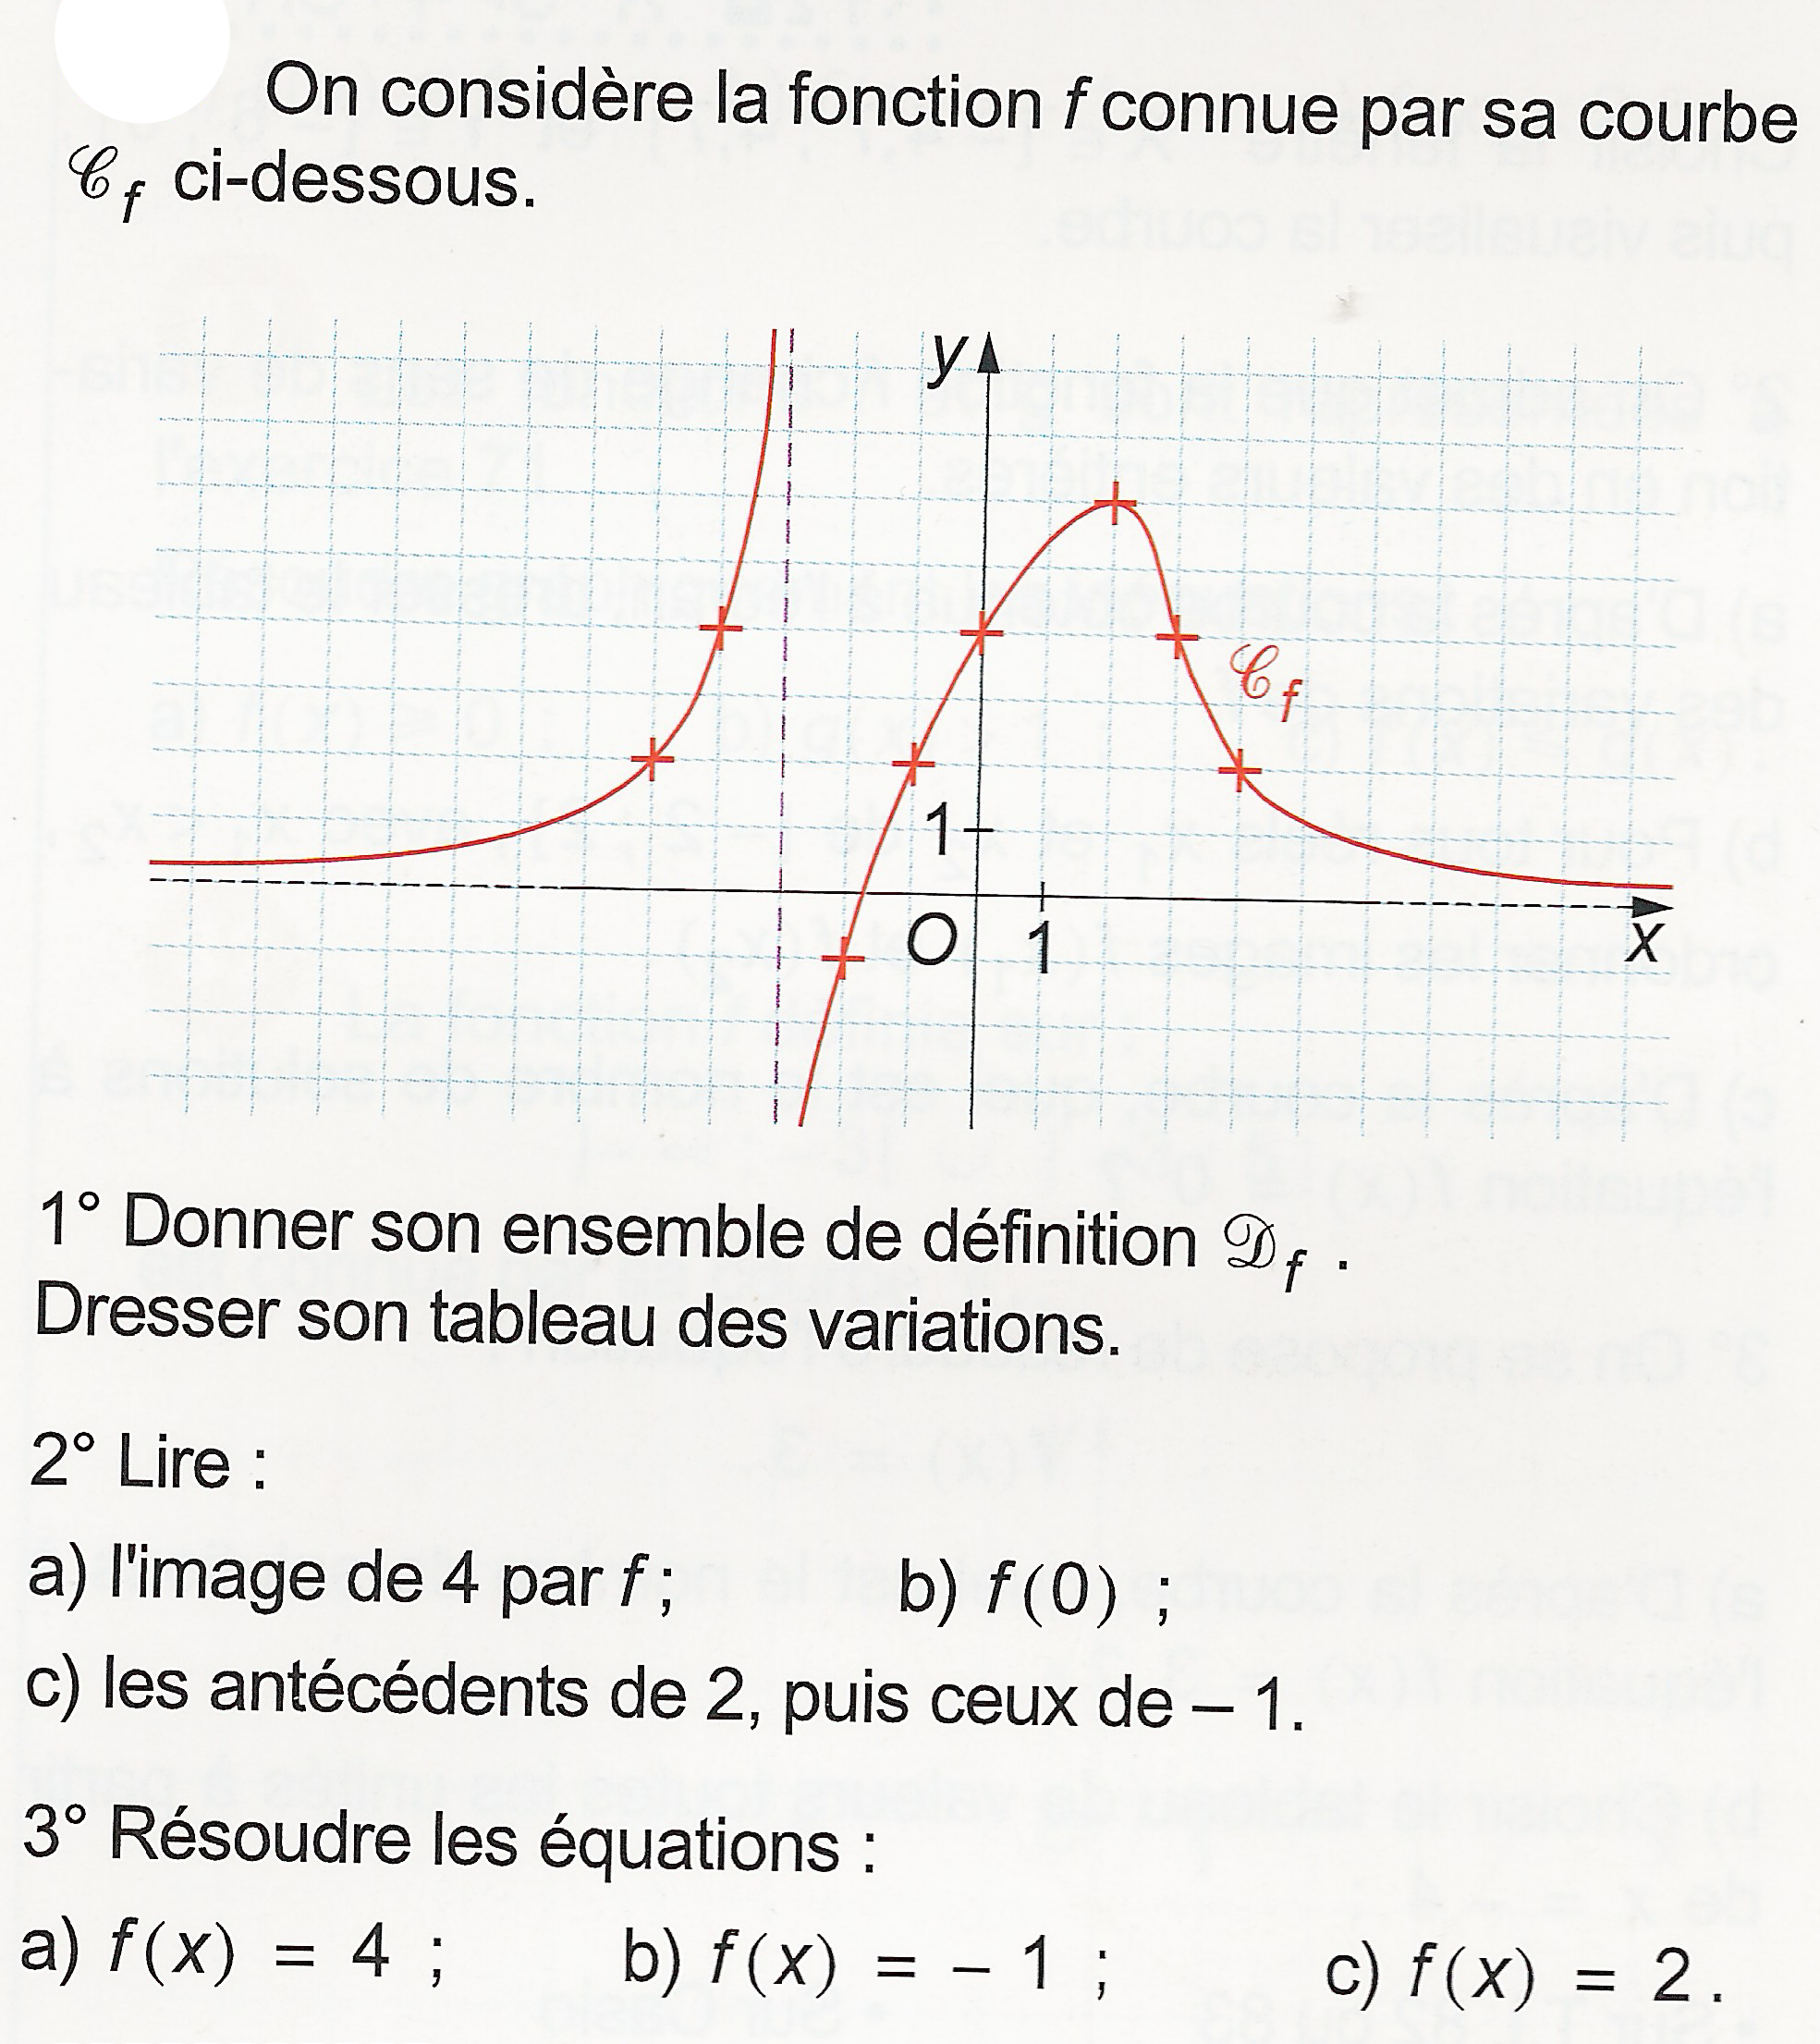
\includegraphics[width=7cm]{images/ex3.png}
\end{minipage} 
&
\begin{minipage}{8cm}
\textbf{Exercice 4}

\enskip


\includegraphics[width=7cm]{images/ex4.png}
\end{minipage}
\end{tabular}
 
 
 \bigskip
 
\begin{tabular}{cc}
\begin{minipage}{7cm}
\textbf{Exercice 5}

\enskip

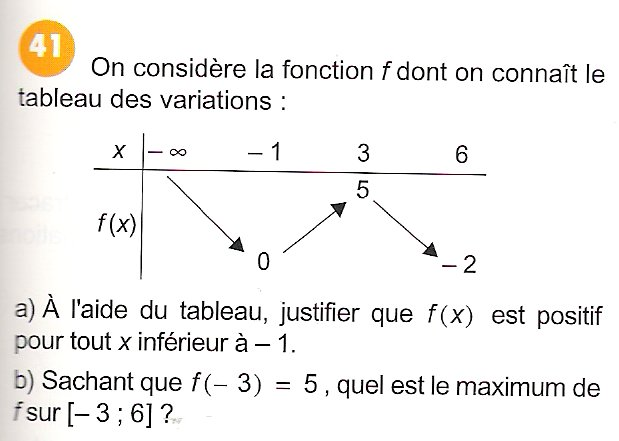
\includegraphics[width=7cm]{images/declic41.jpg}
\end{minipage} 
&
\begin{minipage}{11cm}
\textbf{Exercice 6:} 
\begin{enumerate}
  \item A l'aide de votre calculatrice, conjecturer l'existence d'un extremum
  des fonctions suivantes: $f(x)=x^{2}-7$ \qquad \quad $g(x)=-x^{2}+5$ \qquad
  \quad $h(x)=6+(x-5)^{2}$
  \item D�montrer vos conjectures.
\end{enumerate}

\end{minipage}
\end{tabular}

\bigskip

\textbf{Exercice 7:}
\begin{enumerate}
  \item Montrer que la fonction $f$ d�finie sur $\mathbb{R}$ par $f(x)=5x-100$
  est croissante sur $\mathbb{R}$.
 \item Montrer que la fonction $g$ d�finie sur $\mathbb{R}$ par $g(x)=-2x+3$
  est d�croissante sur $\mathbb{R}$.  
\end{enumerate}

\end{document}
